\section{基本性质}
\label{sec:cexp-properties}

有了定义，下一步是学会运算。在有限分组中，组内平均对随机变量是线性的、保序的，已经知道的量在组内是常数，可以提到平均号外面。这些性质在一般的$\mathcal{G}$下是否仍然成立？本节固定信息$\mathcal{G}$，逐条从积分定义核验它们，并用传感器表检验计算含义。核验的办法都相同：写出候选，检查它$\mathcal{G}$可测、可积，并在每个$A\in\mathcal{G}$上满足式~\eqref{eq:cexp-defining}，再由定理~\ref{thm:cexp-existence}的唯一性得出几乎必然相等。最后讨论另一种极端：当信息与变量独立时，条件平均就是普通的平均。

\subsection{线性与保序}
\label{sec:cexp-linearity}

先看两条最基本的规则。在每一组内求平均，和的平均是平均的和，较大变量的平均不小于较小变量的平均。下面的定理说明它们对一般信息仍然成立，只是相等与不等都按几乎必然理解。

\begin{theorem}[线性与保序]
\label{thm:cexp-linearity}
设$X_1,X_2$可积，$a,b$是实数。则
\begin{equation}
 \mathbb{E}[aX_1+bX_2\mid\mathcal{G}]=a\,\mathbb{E}[X_1\mid\mathcal{G}]+b\,\mathbb{E}[X_2\mid\mathcal{G}].
 \label{eq:cexp-linearity}
\end{equation}
若$X_1\leq X_2$几乎必然成立，则
\begin{equation}
 \mathbb{E}[X_1\mid\mathcal{G}]\leq\mathbb{E}[X_2\mid\mathcal{G}].
 \label{eq:cexp-monotone}
\end{equation}
特别地，常数$c$满足$\mathbb{E}[c\mid\mathcal{G}]=c$，并且
\begin{equation}
 \bigl\lvert\mathbb{E}[X_1\mid\mathcal{G}]\bigr\rvert\leq\mathbb{E}\bigl[\lvert X_1\rvert\bigm|\mathcal{G}\bigr].
 \label{eq:cexp-abs}
\end{equation}
\end{theorem}

\begin{proof}
记$Z_1,Z_2$为$X_1,X_2$的条件期望的版本。

\emph{线性。}$aZ_1+bZ_2$是$\mathcal{G}$可测的可积函数。对$A\in\mathcal{G}$，由期望的线性和式~\eqref{eq:cexp-defining}，
\[
 \mathbb{E}\bigl[(aZ_1+bZ_2)\mathbf{1}_{A}\bigr]
 =a\,\mathbb{E}[X_1\mathbf{1}_{A}]+b\,\mathbb{E}[X_2\mathbf{1}_{A}]
 =\mathbb{E}\bigl[(aX_1+bX_2)\mathbf{1}_{A}\bigr].
\]
所以$aZ_1+bZ_2$是$aX_1+bX_2$的条件期望的一个版本，由唯一性得式~\eqref{eq:cexp-linearity}。

\emph{非负性。}先设$X\geq0$几乎必然成立，$Z$是$\mathbb{E}[X\mid\mathcal{G}]$的版本。事件$A=\{Z<0\}$属于$\mathcal{G}$，于是
\[
 \mathbb{E}[Z\mathbf{1}_{A}]=\mathbb{E}[X\mathbf{1}_{A}]\geq0 .
\]
另一方面$Z\mathbf{1}_{A}\leq0$，期望不大于零。两者合起来，$Z\mathbf{1}_{A}$是期望为零的非正函数，几乎必然为零；它在$A$上严格为负，所以$\mathbb{P}(A)=0$，即$Z\geq0$几乎必然成立。

\emph{保序。}对$X_2-X_1\geq0$用非负性，再用线性，得式~\eqref{eq:cexp-monotone}。由$-\lvert X_1\rvert\leq X_1\leq\lvert X_1\rvert$与保序，得到绝对值的不等式。常数$c$本身是$\mathcal{G}$可测的，满足定义的三条要求。
\end{proof}

线性对应于“组内平均可以逐项计算”，保序对应于“逐点更大的量，组内平均也更大”。在传感器表上，$\mathbb{E}[2Y-1\mid X]=2\,\mathbb{E}[Y\mid X]-1$，三行依次是
\[
 2\cdot\tfrac13-1=-\tfrac13,\qquad 2\cdot1-1=1,\qquad 2\cdot\tfrac53-1=\tfrac73 ,
\]
与直接按行求$2Y-1$的平均相同。又因为$0\leq Y\leq2$，保序给出$0\leq\mathbb{E}[Y\mid X]\leq2$，三个行均值确实落在这个范围。

“几乎必然”在这里有一个实际后果。式~\eqref{eq:cexp-linearity}对每一对$(X_1,X_2)$和每一对系数，都在一个可能依赖于它们的零概率集之外成立。对可数多个这样的等式，把例外集并起来仍是零概率集，可以同时使用；对不可数多个，例如对所有实数$a$同时成立，就不能直接合并例外集。逐事件的条件概率要拼成一个完整的分布，正卡在这一点上，第~\ref{chap:conditional-distributions}章会处理它。

\subsection{提取已知量}
\label{sec:cexp-known}

\paragraph{已知的乘子可以提出}
在一组之内，$\mathcal{G}$可测的量是常数，常数可以从平均里提出来。传感器表中，给定$X$时$X$已知，所以应当有$\mathbb{E}[XY\mid X]=X\,\mathbb{E}[Y\mid X]$。这条规则称为\term{提取已知量}（taking out what is known）。下面的定理说明它对一般信息成立，并说明乘子需要满足什么条件。

\begin{theorem}[提取已知量]
\label{thm:cexp-known}
设$H$是$\mathcal{G}$可测的随机变量，$X$与$HX$都可积。则$H\,\mathbb{E}[X\mid\mathcal{G}]$可积，并且
\begin{equation}
 \mathbb{E}[HX\mid\mathcal{G}]=H\,\mathbb{E}[X\mid\mathcal{G}].
 \label{eq:cexp-known}
\end{equation}
特别地，若$H$是$\mathcal{G}$可测且可积的，则$\mathbb{E}[H\mid\mathcal{G}]=H$。
\end{theorem}

证明分三步扩大乘子的范围：先是示性函数，再是有界函数，最后是一般函数。前两步是定义的直接推论；最后一步的难点在于，事先并不知道$HZ$可积，不能直接用控制收敛定理，需要先对非负的情形用单调收敛定理得到可积性。

\begin{proof}
记$Z=\mathbb{E}[X\mid\mathcal{G}]$。$HZ$是两个$\mathcal{G}$可测函数之积，本身$\mathcal{G}$可测。由唯一性，只需证明$HZ$可积，并且对每个$A\in\mathcal{G}$，
\[
 \mathbb{E}[HX\mathbf{1}_{A}]=\mathbb{E}[HZ\mathbf{1}_{A}] .
\]

\emph{第一步，示性函数与简单函数。}设$H=\mathbf{1}_{B}$，$B\in\mathcal{G}$。$A\cap B\in\mathcal{G}$，由式~\eqref{eq:cexp-defining}，
\[
 \mathbb{E}[\mathbf{1}_{B}X\mathbf{1}_{A}]=\mathbb{E}[X\mathbf{1}_{A\cap B}]=\mathbb{E}[Z\mathbf{1}_{A\cap B}]=\mathbb{E}[\mathbf{1}_{B}Z\mathbf{1}_{A}] .
\]
由线性，结论对$\mathcal{G}$可测的简单函数$H$成立。

\emph{第二步，有界的$H$。}设$\lvert H\rvert\leq c$。取$\mathcal{G}$可测的简单函数$H_n$，使$\lvert H_n\rvert\leq c$且$H_n\to H$逐点成立。由第一步，
\[
 \mathbb{E}[H_nX\mathbf{1}_{A}]=\mathbb{E}[H_nZ\mathbf{1}_{A}] .
\]
左边被积函数被$c\lvert X\rvert$控制，右边被$c\lvert Z\rvert$控制，两者都可积。由控制收敛定理令$n\to\infty$，两边分别趋于$\mathbb{E}[HX\mathbf{1}_{A}]$与$\mathbb{E}[HZ\mathbf{1}_{A}]$。

\emph{第三步，非负的$H$与$X$。}设$H\geq0$，$X\geq0$，于是$Z\geq0$。令$H_n=\min(H,n)$，由第二步，
\[
 \mathbb{E}[H_nX\mathbf{1}_{A}]=\mathbb{E}[H_nZ\mathbf{1}_{A}] .
\]
两边的被积函数都非负并且随$n$单调增加，由单调收敛定理令$n\to\infty$，得到
\[
 \mathbb{E}[HX\mathbf{1}_{A}]=\mathbb{E}[HZ\mathbf{1}_{A}] .
\]
取$A=\Omega$，左边是有限的$\mathbb{E}[HX]$，所以$HZ$可积。

\emph{第四步，一般情形。}写$H=H^{+}-H^{-}$，$X=X^{+}-X^{-}$，并记$Z_{\pm}=\mathbb{E}[X^{\pm}\mid\mathcal{G}]$，于是$Z=Z_{+}-Z_{-}$。四个乘积$H^{\pm}X^{\pm}$都被$\lvert HX\rvert$控制，因而可积。对每一对符号用第三步，得到$H^{\pm}Z_{\pm}$可积，且
\[
 \mathbb{E}[H^{\pm}X^{\pm}\mathbf{1}_{A}]=\mathbb{E}[H^{\pm}Z_{\pm}\mathbf{1}_{A}] .
\]
把四个等式按$HX=(H^{+}-H^{-})(X^{+}-X^{-})$的符号相加，右边合成$\mathbb{E}[HZ\mathbf{1}_{A}]$，左边合成$\mathbb{E}[HX\mathbf{1}_{A}]$；而$\lvert HZ\rvert$不超过四个可积函数$H^{\pm}Z_{\pm}$之和，所以$HZ$可积。

最后一句取$X=1$：$\mathbb{E}[1\mid\mathcal{G}]=1$，$H\cdot1$可积，于是$\mathbb{E}[H\mid\mathcal{G}]=H$。
\end{proof}

定理要求$HX$可积，否则左边的条件期望在本章的意义下没有定义。乘子本身不必有界：$X$与$HX$可积就够了，结论里$H\,\mathbb{E}[X\mid\mathcal{G}]$的可积性是证明出来的，不是假设的。

\paragraph{传感器表上的计算}
在传感器表中取$H=X$，它是$\sigma(X)$可测的。由式~\eqref{eq:cexp-known}与三行的条件均值，
\[
 \mathbb{E}[XY\mid X]=X\,\mathbb{E}[Y\mid X]:\qquad 0\cdot\tfrac13=0,\qquad 1\cdot1=1,\qquad 2\cdot\tfrac53=\tfrac{10}{3},
\]
见图~\ref{fig:cexp-known-factor}(a)。直接计算第三行核对：第三行中$Y$以条件概率$\tfrac13,\tfrac23$取$1,2$，$XY$取$2,4$，平均为$\tfrac23+\tfrac83=\tfrac{10}{3}$。

\begin{BookInlineFigure}
  \centering
  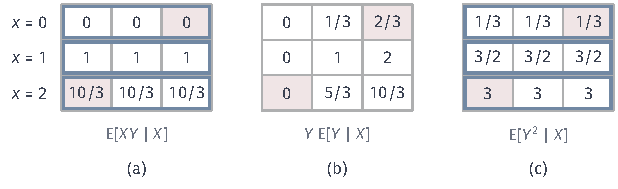
\includegraphics[width=104mm]{figures/07-probability/02-measure-theoretic-probability/tikz/cexp-known-factor/figure.pdf}
  \caption{提取已知量，传感器表，浅红格的概率为零。(a)$\mathbb{E}[XY\mid X]=X\,\mathbb{E}[Y\mid X]$，每行取常数$0$、$1$、$10/3$（蓝框表示行内为常数）。(b)$Y\,\mathbb{E}[Y\mid X]$在同一行内变化，不是$X$的函数。(c)$\mathbb{E}[Y^{2}\mid X]$，每行取$1/3$、$3/2$、$3$。}
  \label{fig:cexp-known-factor}
\end{BookInlineFigure}

\paragraph{未知的乘子不能提出}
乘子必须是已知的。若把$Y$当作乘子，“$\mathbb{E}[Y\cdot Y\mid X]=Y\,\mathbb{E}[Y\mid X]$”就是错的。右边在同一行内随$Y$变化，见图~\ref{fig:cexp-known-factor}(b)，它不是$\sigma(X)$可测的，根本不可能是给定$X$的条件期望。正确的值由行内平均给出：
\[
 \mathbb{E}[Y^{2}\mid X=0]=\tfrac13,\qquad \mathbb{E}[Y^{2}\mid X=1]=\tfrac32,\qquad \mathbb{E}[Y^{2}\mid X=2]=3 ,
\]
见图~\ref{fig:cexp-known-factor}(c)。例如第二行中$Y^{2}$以$\tfrac14,\tfrac12,\tfrac14$取$0,1,4$，平均为$\tfrac12+1=\tfrac32$。在组内，已知量是常数，未知量仍在变化；只有前者能提到平均号外面。

\subsection{独立情形}
\label{sec:cexp-independence}

\paragraph{与信息独立的变量}
如果已知的信息与$X$毫无关联，给定这份信息的平均就不应改变。称$X$与$\mathcal{G}$独立，是指对每个Borel集$B$与每个$A\in\mathcal{G}$，事件$\{X\in B\}$与$A$独立，也就是$\sigma(X)$与$\mathcal{G}$独立。这时$X$与每个$\mathbf{1}_{A}$是独立的随机变量，由第~\ref{chap:probability-spaces}章的积分表示，两个独立可积变量乘积的期望等于期望的乘积。

\begin{theorem}[独立的信息]
\label{thm:cexp-independent}
设$X$可积并且与$\mathcal{G}$独立。则
\begin{equation}
 \mathbb{E}[X\mid\mathcal{G}]=\mathbb{E}[X].
 \label{eq:cexp-independent}
\end{equation}
\end{theorem}

\begin{proof}
常数$\mathbb{E}[X]$是$\mathcal{G}$可测且可积的。对$A\in\mathcal{G}$，$X$与$\mathbf{1}_{A}$独立且都可积，乘积的期望等于期望的乘积，
\[
 \mathbb{E}[X\mathbf{1}_{A}]=\mathbb{E}[X]\,\mathbb{P}(A)=\mathbb{E}\bigl[\mathbb{E}[X]\,\mathbf{1}_{A}\bigr].
\]
所以常数$\mathbb{E}[X]$满足式~\eqref{eq:cexp-defining}。
\end{proof}

“只知绝对值”的例子提供了一个独立的情形。记$S=\operatorname{sgn}X$，它以各$\tfrac12$的概率取$\pm1$。对$0\leq t\leq1$，
\[
 \mathbb{P}\bigl(S=1,\ \lvert X\rvert\leq t\bigr)=\mathbb{P}(0<X\leq t)=\frac t2=\mathbb{P}(S=1)\,\mathbb{P}\bigl(\lvert X\rvert\leq t\bigr),
\]
所以符号与绝对值独立。由定理~\ref{thm:cexp-independent}，$\mathbb{E}[S\mid\lvert X\rvert]=\mathbb{E}[S]=0$：知道离原点多远，对“在哪一侧”毫无帮助。再由$X=S\lvert X\rvert$与提取已知量，
\[
 \mathbb{E}\bigl[X\bigm|\lvert X\rvert\bigr]=\lvert X\rvert\,\mathbb{E}\bigl[S\bigm|\lvert X\rvert\bigr]=0 ,
\]
与式~\eqref{eq:cexp-folding}取$g(x)=x$的结果一致。

\paragraph{条件平均为常数不能推出独立}
定理~\ref{thm:cexp-independent}的逆命题不成立。上面刚得到$\mathbb{E}[X\mid\lvert X\rvert]=0=\mathbb{E}[X]$，可是$X$与$\lvert X\rvert$不独立，取一对事件就能看出：
\[
 \mathbb{P}\bigl(\lvert X\rvert\leq\tfrac12,\ X>\tfrac12\bigr)=0,\qquad
 \mathbb{P}\bigl(\lvert X\rvert\leq\tfrac12\bigr)\,\mathbb{P}\bigl(X>\tfrac12\bigr)=\tfrac12\cdot\tfrac14=\tfrac18 .
\]
图~\ref{fig:cexp-independence}比较了两种情形。左边给定$\lvert X\rvert=y$后，$X$只能是$\pm y$，条件规律随$y$剧烈变化，只是两点的平均恰好总为$0$；右边$Z$与$X$独立，给定$Z$后$X$的整个分布都不变。两者的条件平均都是常数$0$，图中的红线完全相同。

\begin{BookInlineFigure}
  \centering
  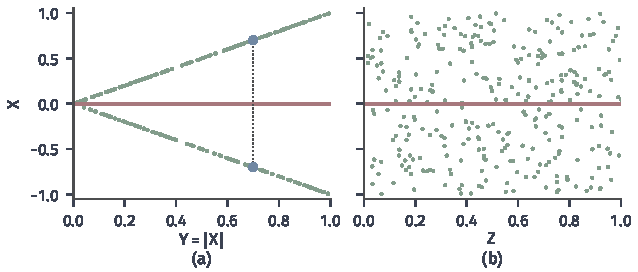
\includegraphics[width=108mm]{figures/07-probability/02-measure-theoretic-probability/matplotlib/cexp-independence/figure.pdf}
  \caption{条件平均为常数不等于独立。随机数种子$7$，各$300$个模拟点（绿）。(a)$X\sim\operatorname{Unif}(-1,1)$与$Y=\lvert X\rvert$，点落在两条线段$x=\pm y$上；给定$Y=0.7$时$X$只取蓝点$\pm0.7$，条件平均为$0$（红线）。(b)$X\sim\operatorname{Unif}(-1,1)$与独立的$Z\sim\operatorname{Unif}(0,1)$，点铺满矩形，条件平均同样为$0$。}
  \label{fig:cexp-independence}
\end{BookInlineFigure}

条件平均为常数只约束一个数：每组的平均都等于总平均。独立则要求给定信息后$X$落在任何集合中的条件概率都不变，即对一切Borel集$B$，
\[
 \mathbb{E}\bigl[\mathbf{1}_{\{X\in B\}}\bigm|\mathcal{G}\bigr]=\mathbb{P}(X\in B).
\]
前者只要求$X$本身的条件平均不变，后者要求每个示性函数$\mathbf{1}_{\{X\in B\}}$的条件平均都不变，由后者可以推出前者。给定信息后完整的条件规律在第~\ref{chap:conditional-distributions}章研究，那里的条件独立也要求整个条件分布满足乘积关系，而不只是条件均值。
